\documentclass[1p]{elsarticle_modified}
%\bibliographystyle{elsarticle-num}

%\usepackage[colorlinks]{hyperref}
%\usepackage{abbrmath_seonhwa} %\Abb, \Ascr, \Acal ,\Abf, \Afrak
\usepackage{amsfonts}
\usepackage{amssymb}
\usepackage{amsmath}
\usepackage{amsthm}
\usepackage{scalefnt}
\usepackage{amsbsy}
\usepackage{kotex}
\usepackage{caption}
\usepackage{subfig}
\usepackage{color}
\usepackage{graphicx}
\usepackage{xcolor} %% white, black, red, green, blue, cyan, magenta, yellow
\usepackage{float}
\usepackage{setspace}
\usepackage{hyperref}

\usepackage{tikz}
\usetikzlibrary{arrows}

\usepackage{multirow}
\usepackage{array} % fixed length table
\usepackage{hhline}

%%%%%%%%%%%%%%%%%%%%%
\makeatletter
\renewcommand*\env@matrix[1][\arraystretch]{%
	\edef\arraystretch{#1}%
	\hskip -\arraycolsep
	\let\@ifnextchar\new@ifnextchar
	\array{*\c@MaxMatrixCols c}}
\makeatother %https://tex.stackexchange.com/questions/14071/how-can-i-increase-the-line-spacing-in-a-matrix
%%%%%%%%%%%%%%%

\usepackage[normalem]{ulem}

\newcommand{\msout}[1]{\ifmmode\text{\sout{\ensuremath{#1}}}\else\sout{#1}\fi}
%SOURCE: \msout is \stkout macro in https://tex.stackexchange.com/questions/20609/strikeout-in-math-mode

\newcommand{\cancel}[1]{
	\ifmmode
	{\color{red}\msout{#1}}
	\else
	{\color{red}\sout{#1}}
	\fi
}

\newcommand{\add}[1]{
	{\color{blue}\uwave{#1}}
}

\newcommand{\replace}[2]{
	\ifmmode
	{\color{red}\msout{#1}}{\color{blue}\uwave{#2}}
	\else
	{\color{red}\sout{#1}}{\color{blue}\uwave{#2}}
	\fi
}

\newcommand{\Sol}{\mathcal{S}} %segment
\newcommand{\D}{D} %diagram
\newcommand{\A}{\mathcal{A}} %arc


%%%%%%%%%%%%%%%%%%%%%%%%%%%%%5 test

\def\sl{\operatorname{\textup{SL}}(2,\Cbb)}
\def\psl{\operatorname{\textup{PSL}}(2,\Cbb)}
\def\quan{\mkern 1mu \triangleright \mkern 1mu}

\theoremstyle{definition}
\newtheorem{thm}{Theorem}[section]
\newtheorem{prop}[thm]{Proposition}
\newtheorem{lem}[thm]{Lemma}
\newtheorem{ques}[thm]{Question}
\newtheorem{cor}[thm]{Corollary}
\newtheorem{defn}[thm]{Definition}
\newtheorem{exam}[thm]{Example}
\newtheorem{rmk}[thm]{Remark}
\newtheorem{alg}[thm]{Algorithm}

\newcommand{\I}{\sqrt{-1}}
\begin{document}

%\begin{frontmatter}
%
%\title{Boundary parabolic representations of knots up to 8 crossings}
%
%%% Group authors per affiliation:
%\author{Yunhi Cho} 
%\address{Department of Mathematics, University of Seoul, Seoul, Korea}
%\ead{yhcho@uos.ac.kr}
%
%
%\author{Seonhwa Kim} %\fnref{s_kim}}
%\address{Center for Geometry and Physics, Institute for Basic Science, Pohang, 37673, Korea}
%\ead{ryeona17@ibs.re.kr}
%
%\author{Hyuk Kim}
%\address{Department of Mathematical Sciences, Seoul National University, Seoul 08826, Korea}
%\ead{hyukkim@snu.ac.kr}
%
%\author{Seokbeom Yoon}
%\address{Department of Mathematical Sciences, Seoul National University, Seoul, 08826,  Korea}
%\ead{sbyoon15@snu.ac.kr}
%
%\begin{abstract}
%We find all boundary parabolic representation of knots up to 8 crossings.
%
%\end{abstract}
%\begin{keyword}
%    \MSC[2010] 57M25 
%\end{keyword}
%
%\end{frontmatter}

%\linenumbers
%\tableofcontents
%
\newcommand\colored[1]{\textcolor{white}{\rule[-0.35ex]{0.8em}{1.4ex}}\kern-0.8em\color{red} #1}%
%\newcommand\colored[1]{\textcolor{white}{ #1}\kern-2.17ex	\textcolor{white}{ #1}\kern-1.81ex	\textcolor{white}{ #1}\kern-2.15ex\color{red}#1	}

{\Large $\underline{12n_{0660}~(K12n_{0660})}$}

\setlength{\tabcolsep}{10pt}
\renewcommand{\arraystretch}{1.6}
\vspace{1cm}\begin{tabular}{m{100pt}>{\centering\arraybackslash}m{274pt}}
\multirow{5}{120pt}{
	\centering
	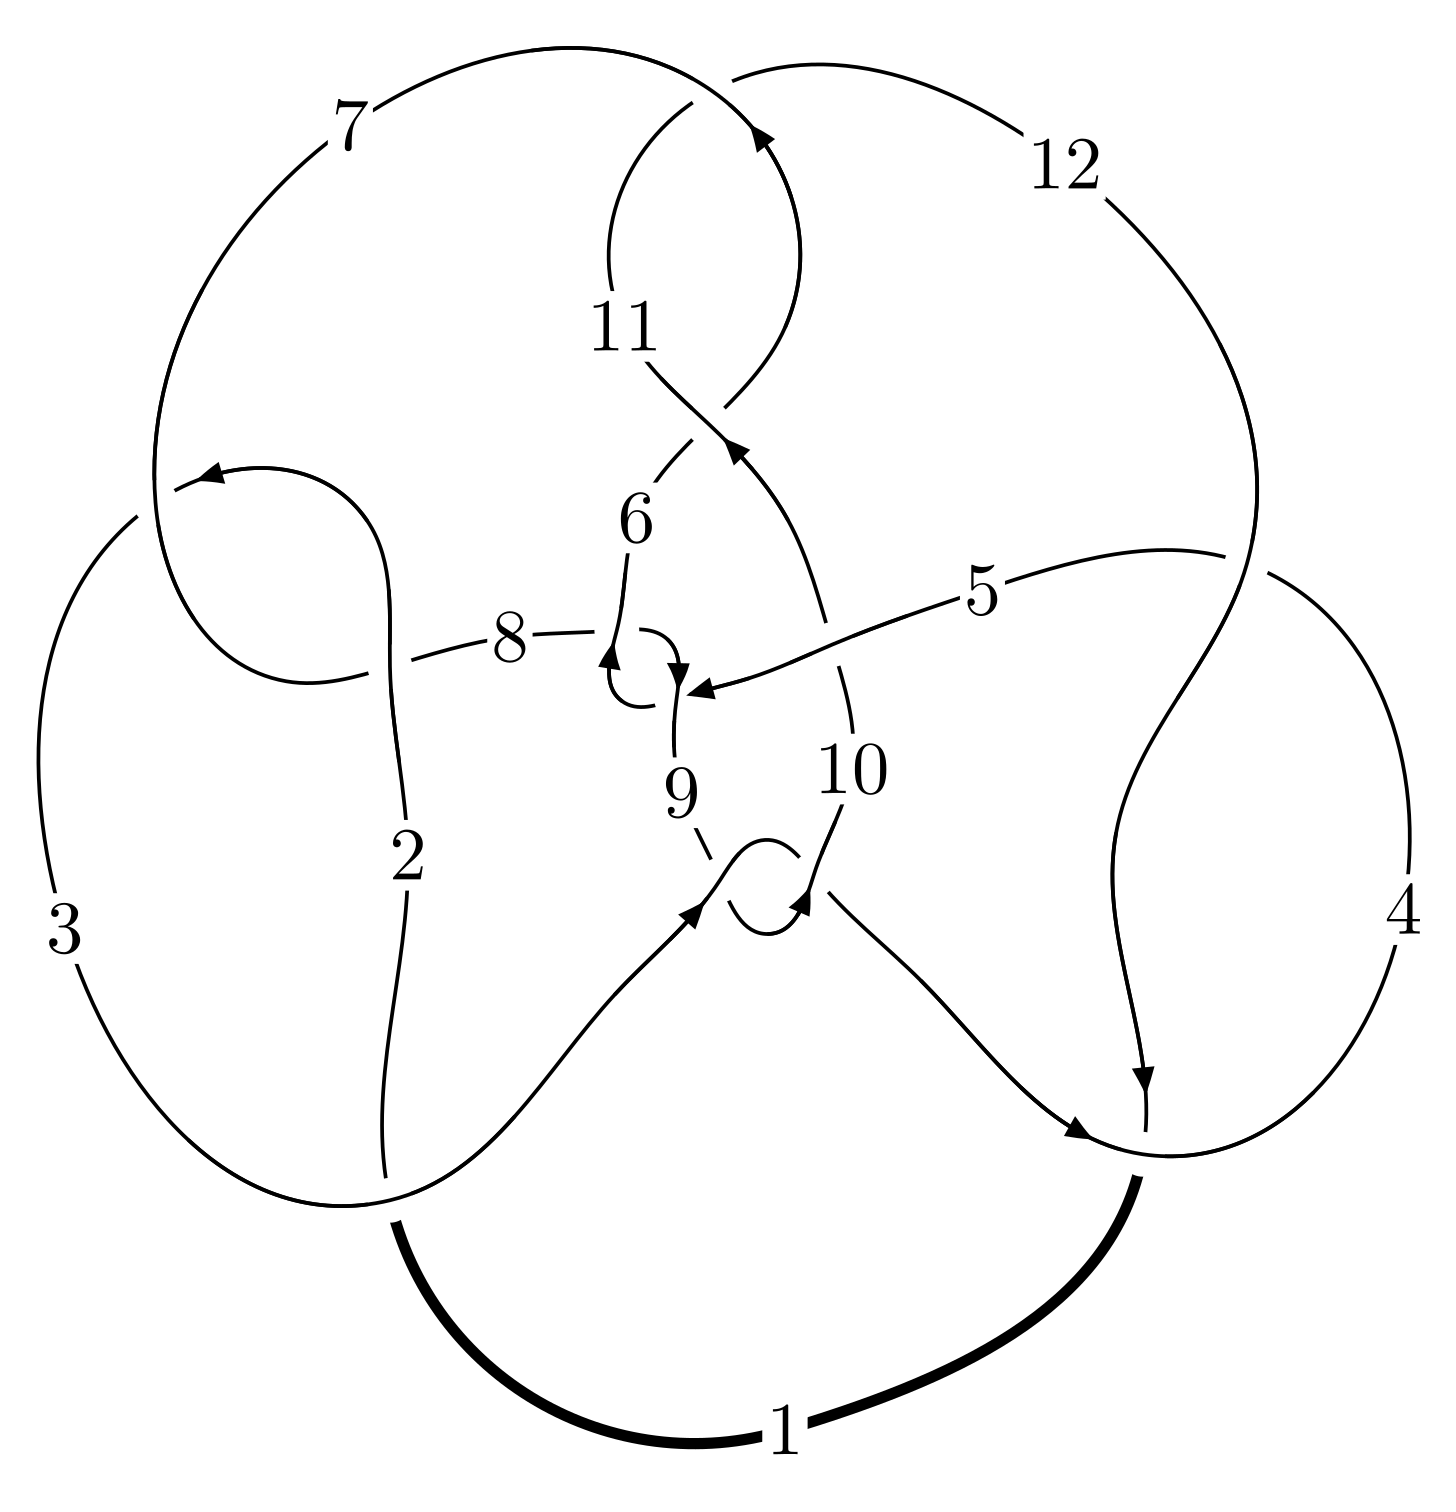
\includegraphics[width=112pt]{../../../GIT/diagram.site/Diagrams/png/2749_12n_0660.png}\\
\ \ \ A knot diagram\footnotemark}&
\allowdisplaybreaks
\textbf{Linearized knot diagam} \\
\cline{2-2}
 &
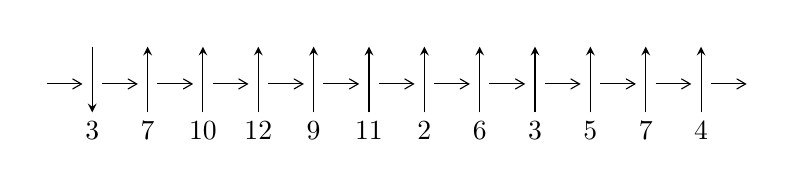
\begin{tikzpicture}[x=20pt, y=17pt]
	% nodes
	\node (C0) at (0, 0) {};
	\node (C1) at (1, 0) {};
	\node (C1U) at (1, +1) {};
	\node (C1D) at (1, -1) {3};

	\node (C2) at (2, 0) {};
	\node (C2U) at (2, +1) {};
	\node (C2D) at (2, -1) {7};

	\node (C3) at (3, 0) {};
	\node (C3U) at (3, +1) {};
	\node (C3D) at (3, -1) {10};

	\node (C4) at (4, 0) {};
	\node (C4U) at (4, +1) {};
	\node (C4D) at (4, -1) {12};

	\node (C5) at (5, 0) {};
	\node (C5U) at (5, +1) {};
	\node (C5D) at (5, -1) {9};

	\node (C6) at (6, 0) {};
	\node (C6U) at (6, +1) {};
	\node (C6D) at (6, -1) {11};

	\node (C7) at (7, 0) {};
	\node (C7U) at (7, +1) {};
	\node (C7D) at (7, -1) {2};

	\node (C8) at (8, 0) {};
	\node (C8U) at (8, +1) {};
	\node (C8D) at (8, -1) {6};

	\node (C9) at (9, 0) {};
	\node (C9U) at (9, +1) {};
	\node (C9D) at (9, -1) {3};

	\node (C10) at (10, 0) {};
	\node (C10U) at (10, +1) {};
	\node (C10D) at (10, -1) {5};

	\node (C11) at (11, 0) {};
	\node (C11U) at (11, +1) {};
	\node (C11D) at (11, -1) {7};

	\node (C12) at (12, 0) {};
	\node (C12U) at (12, +1) {};
	\node (C12D) at (12, -1) {4};
	\node (C13) at (13, 0) {};

	% arrows
	\draw[->,>={angle 60}]
	(C0) edge (C1) (C1) edge (C2) (C2) edge (C3) (C3) edge (C4) (C4) edge (C5) (C5) edge (C6) (C6) edge (C7) (C7) edge (C8) (C8) edge (C9) (C9) edge (C10) (C10) edge (C11) (C11) edge (C12) (C12) edge (C13) ;	\draw[->,>=stealth]
	(C1U) edge (C1D) (C2D) edge (C2U) (C3D) edge (C3U) (C4D) edge (C4U) (C5D) edge (C5U) (C6D) edge (C6U) (C7D) edge (C7U) (C8D) edge (C8U) (C9D) edge (C9U) (C10D) edge (C10U) (C11D) edge (C11U) (C12D) edge (C12U) ;
	\end{tikzpicture} \\
\hhline{~~} \\& 
\textbf{Solving Sequence} \\ \cline{2-2} 
 &
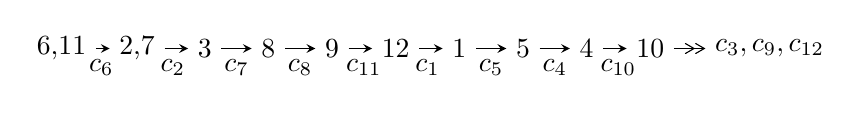
\begin{tikzpicture}[x=23pt, y=7pt]
	% node
	\node (A0) at (-1/8, 0) {6,11};
	\node (A1) at (17/16, 0) {2,7};
	\node (A2) at (17/8, 0) {3};
	\node (A3) at (25/8, 0) {8};
	\node (A4) at (33/8, 0) {9};
	\node (A5) at (41/8, 0) {12};
	\node (A6) at (49/8, 0) {1};
	\node (A7) at (57/8, 0) {5};
	\node (A8) at (65/8, 0) {4};
	\node (A9) at (73/8, 0) {10};
	\node (C1) at (1/2, -1) {$c_{6}$};
	\node (C2) at (13/8, -1) {$c_{2}$};
	\node (C3) at (21/8, -1) {$c_{7}$};
	\node (C4) at (29/8, -1) {$c_{8}$};
	\node (C5) at (37/8, -1) {$c_{11}$};
	\node (C6) at (45/8, -1) {$c_{1}$};
	\node (C7) at (53/8, -1) {$c_{5}$};
	\node (C8) at (61/8, -1) {$c_{4}$};
	\node (C9) at (69/8, -1) {$c_{10}$};
	\node (A10) at (11, 0) {$c_{3},c_{9},c_{12}$};

	% edge
	\draw[->,>=stealth]	
	(A0) edge (A1) (A1) edge (A2) (A2) edge (A3) (A3) edge (A4) (A4) edge (A5) (A5) edge (A6) (A6) edge (A7) (A7) edge (A8) (A8) edge (A9) ;
	\draw[->>,>={angle 60}]	
	(A9) edge (A10);
\end{tikzpicture} \\ 

\end{tabular} \\

\footnotetext{
The image of knot diagram is generated by the software ``\textbf{Draw programme}" developed by Andrew Bartholomew(\url{http://www.layer8.co.uk/maths/draw/index.htm\#Running-draw}), where we modified some parts for our purpose(\url{https://github.com/CATsTAILs/LinksPainter}).
}\phantom \\ \newline 
\centering \textbf{Ideals for irreducible components\footnotemark of $X_{\text{par}}$} 
 
\begin{align*}
I^u_{1}&=\langle 
-11564599 u^{15}-9251046 u^{14}+\cdots+53220158 b+13391876,\\
\phantom{I^u_{1}}&\phantom{= \langle  }-43861146 u^{15}-59898749 u^{14}+\cdots+53220158 a-99727540,\\
\phantom{I^u_{1}}&\phantom{= \langle  }u^{16}+u^{15}+u^{14}+2 u^{13}+9 u^{12}+9 u^{11}+16 u^{10}+9 u^9+8 u^8+19 u^7-33 u^6-6 u^5+3 u^4-33 u^3+4 u^2+3 u-1\rangle \\
I^u_{2}&=\langle 
-1.75232\times10^{59} u^{33}+3.07107\times10^{59} u^{32}+\cdots+1.28337\times10^{61} b+1.83553\times10^{61},\\
\phantom{I^u_{2}}&\phantom{= \langle  }1.93452\times10^{60} u^{33}-1.32279\times10^{60} u^{32}+\cdots+1.28337\times10^{61} a-1.86396\times10^{62},\;u^{34}- u^{33}+\cdots-180 u-3\rangle \\
I^u_{3}&=\langle 
1.97277\times10^{16} u^{25}+6.79934\times10^{15} u^{24}+\cdots+1.89124\times10^{16} b+5.92285\times10^{16},\\
\phantom{I^u_{3}}&\phantom{= \langle  }6.86300\times10^{15} u^{25}-1.50215\times10^{16} u^{24}+\cdots+1.89124\times10^{16} a-1.96975\times10^{16},\;u^{26}-8 u^{24}+\cdots+4 u-1\rangle \\
I^u_{4}&=\langle 
- u^2+b-1,\;a- u+1,\;u^3+u+1\rangle \\
I^u_{5}&=\langle 
b-1,\;a+1,\;u-1\rangle \\
\\
\end{align*}
\raggedright * 5 irreducible components of $\dim_{\mathbb{C}}=0$, with total 80 representations.\\
\footnotetext{All coefficients of polynomials are rational numbers. But the coefficients are sometimes approximated in decimal forms when there is not enough margin.}
\newpage
\renewcommand{\arraystretch}{1}
\centering \section*{I. $I^u_{1}= \langle -1.16\times10^{7} u^{15}-9.25\times10^{6} u^{14}+\cdots+5.32\times10^{7} b+1.34\times10^{7},\;-4.39\times10^{7} u^{15}-5.99\times10^{7} u^{14}+\cdots+5.32\times10^{7} a-9.97\times10^{7},\;u^{16}+u^{15}+\cdots+3 u-1 \rangle$}
\flushleft \textbf{(i) Arc colorings}\\
\begin{tabular}{m{7pt} m{180pt} m{7pt} m{180pt} }
\flushright $a_{6}=$&$\begin{pmatrix}1\\0\end{pmatrix}$ \\
\flushright $a_{11}=$&$\begin{pmatrix}0\\u\end{pmatrix}$ \\
\flushright $a_{2}=$&$\begin{pmatrix}0.824145 u^{15}+1.12549 u^{14}+\cdots-7.08904 u+1.87387\\0.217297 u^{15}+0.173826 u^{14}+\cdots-2.02601 u-0.251632\end{pmatrix}$ \\
\flushright $a_{7}=$&$\begin{pmatrix}1\\- u^2\end{pmatrix}$ \\
\flushright $a_{3}=$&$\begin{pmatrix}1.07004 u^{15}+1.41983 u^{14}+\cdots-9.19494 u+1.92358\\0.105243 u^{15}+0.195897 u^{14}+\cdots-2.12657 u-0.300078\end{pmatrix}$ \\
\flushright $a_{8}=$&$\begin{pmatrix}1.10638 u^{15}+1.15362 u^{14}+\cdots-1.22536 u+4.57509\\0.295873 u^{15}+0.428955 u^{14}+\cdots-1.45986 u+0.643823\end{pmatrix}$ \\
\flushright $a_{9}=$&$\begin{pmatrix}1.40226 u^{15}+1.58258 u^{14}+\cdots-2.68521 u+5.21891\\0.295873 u^{15}+0.428955 u^{14}+\cdots-1.45986 u+0.643823\end{pmatrix}$ \\
\flushright $a_{12}=$&$\begin{pmatrix}u\\- u^3+u\end{pmatrix}$ \\
\flushright $a_{1}=$&$\begin{pmatrix}1.32715 u^{15}+1.46973 u^{14}+\cdots-2.19396 u+5.38564\\0.376362 u^{15}+0.378182 u^{14}+\cdots-2.77171 u+0.956452\end{pmatrix}$ \\
\flushright $a_{5}=$&$\begin{pmatrix}0.615985 u^{15}+1.01147 u^{14}+\cdots-9.98396 u-0.124338\\-0.166727 u^{15}-0.0916225 u^{14}+\cdots-1.31231 u-0.991434\end{pmatrix}$ \\
\flushright $a_{4}=$&$\begin{pmatrix}0.749067 u^{15}+1.13559 u^{14}+\cdots-10.2278 u+0.171535\\-0.0503356 u^{15}+0.0874600 u^{14}+\cdots-1.71606 u-0.686604\end{pmatrix}$ \\
\flushright $a_{10}=$&$\begin{pmatrix}1.75205 u^{15}+2.07302 u^{14}+\cdots-3.97175 u+6.28895\\0.386527 u^{15}+0.542106 u^{14}+\cdots-2.07567 u+0.749067\end{pmatrix}$\\&\end{tabular}
\flushleft \textbf{(ii) Obstruction class $= -1$}\\~\\
\flushleft \textbf{(iii) Cusp Shapes $= \frac{40466911}{53220158} u^{15}+\frac{23371529}{26610079} u^{14}+\cdots-\frac{846110475}{53220158} u+\frac{684608261}{53220158}$}\\~\\
\newpage\renewcommand{\arraystretch}{1}
\flushleft \textbf{(iv) u-Polynomials at the component}\newline \\
\begin{tabular}{m{50pt}|m{274pt}}
Crossings & \hspace{64pt}u-Polynomials at each crossing \\
\hline $$\begin{aligned}c_{1}\end{aligned}$$&$\begin{aligned}
&u^{16}+15 u^{15}+\cdots-732 u+16
\end{aligned}$\\
\hline $$\begin{aligned}c_{2},c_{7}\end{aligned}$$&$\begin{aligned}
&u^{16}+5 u^{15}+\cdots-30 u+4
\end{aligned}$\\
\hline $$\begin{aligned}c_{3},c_{6},c_{9}\\c_{11}\end{aligned}$$&$\begin{aligned}
&u^{16}- u^{15}+\cdots-3 u-1
\end{aligned}$\\
\hline $$\begin{aligned}c_{4},c_{5},c_{8}\\c_{12}\end{aligned}$$&$\begin{aligned}
&u^{16}+2 u^{15}+\cdots+2 u+3
\end{aligned}$\\
\hline $$\begin{aligned}c_{10}\end{aligned}$$&$\begin{aligned}
&u^{16}-6 u^{15}+\cdots+32 u-32
\end{aligned}$\\
\hline
\end{tabular}\\~\\
\newpage\renewcommand{\arraystretch}{1}
\flushleft \textbf{(v) Riley Polynomials at the component}\newline \\
\begin{tabular}{m{50pt}|m{274pt}}
Crossings & \hspace{64pt}Riley Polynomials at each crossing \\
\hline $$\begin{aligned}c_{1}\end{aligned}$$&$\begin{aligned}
&y^{16}-25 y^{15}+\cdots-540400 y+256
\end{aligned}$\\
\hline $$\begin{aligned}c_{2},c_{7}\end{aligned}$$&$\begin{aligned}
&y^{16}+15 y^{15}+\cdots-732 y+16
\end{aligned}$\\
\hline $$\begin{aligned}c_{3},c_{6},c_{9}\\c_{11}\end{aligned}$$&$\begin{aligned}
&y^{16}+y^{15}+\cdots-17 y+1
\end{aligned}$\\
\hline $$\begin{aligned}c_{4},c_{5},c_{8}\\c_{12}\end{aligned}$$&$\begin{aligned}
&y^{16}+22 y^{15}+\cdots-130 y+9
\end{aligned}$\\
\hline $$\begin{aligned}c_{10}\end{aligned}$$&$\begin{aligned}
&y^{16}+2 y^{15}+\cdots-12288 y+1024
\end{aligned}$\\
\hline
\end{tabular}\\~\\
\newpage\flushleft \textbf{(vi) Complex Volumes and Cusp Shapes}
$$\begin{array}{c|c|c}  
\text{Solutions to }I^u_{1}& \I (\text{vol} + \sqrt{-1}CS) & \text{Cusp shape}\\
 \hline 
\begin{aligned}
u &= \phantom{-}0.304353 + 0.972075 I \\
a &= \phantom{-}0.50278 - 1.51617 I \\
b &= -0.285550 - 0.101448 I\end{aligned}
 & -4.22498 + 1.58731 I & \phantom{-}9.57126 - 4.28514 I \\ \hline\begin{aligned}
u &= \phantom{-}0.304353 - 0.972075 I \\
a &= \phantom{-}0.50278 + 1.51617 I \\
b &= -0.285550 + 0.101448 I\end{aligned}
 & -4.22498 - 1.58731 I & \phantom{-}9.57126 + 4.28514 I \\ \hline\begin{aligned}
u &= \phantom{-}0.963344\phantom{ +0.000000I} \\
a &= -1.08170\phantom{ +0.000000I} \\
b &= \phantom{-}1.15231\phantom{ +0.000000I}\end{aligned}
 & \phantom{-}4.93639\phantom{ +0.000000I} & \phantom{-}18.2520\phantom{ +0.000000I} \\ \hline\begin{aligned}
u &= -1.113490 + 0.020930 I \\
a &= -1.059080 - 0.259286 I \\
b &= \phantom{-}0.93667 + 1.24298 I\end{aligned}
 & \phantom{-}3.10928 - 2.74603 I & \phantom{-}11.38606 + 5.54848 I \\ \hline\begin{aligned}
u &= -1.113490 - 0.020930 I \\
a &= -1.059080 + 0.259286 I \\
b &= \phantom{-}0.93667 - 1.24298 I\end{aligned}
 & \phantom{-}3.10928 + 2.74603 I & \phantom{-}11.38606 - 5.54848 I \\ \hline\begin{aligned}
u &= \phantom{-}0.431687 + 1.044540 I \\
a &= \phantom{-}1.081630 - 0.710533 I \\
b &= \phantom{-}0.548841 - 0.957392 I\end{aligned}
 & -5.91455 + 0.25172 I & \phantom{-}1.47661 + 0.31305 I \\ \hline\begin{aligned}
u &= \phantom{-}0.431687 - 1.044540 I \\
a &= \phantom{-}1.081630 + 0.710533 I \\
b &= \phantom{-}0.548841 + 0.957392 I\end{aligned}
 & -5.91455 - 0.25172 I & \phantom{-}1.47661 - 0.31305 I \\ \hline\begin{aligned}
u &= -0.50668 + 1.37706 I \\
a &= -0.002750 - 0.610446 I \\
b &= -1.002360 - 0.102183 I\end{aligned}
 & -8.11817 - 5.61695 I & \phantom{-}5.09400 + 3.95642 I \\ \hline\begin{aligned}
u &= -0.50668 - 1.37706 I \\
a &= -0.002750 + 0.610446 I \\
b &= -1.002360 + 0.102183 I\end{aligned}
 & -8.11817 + 5.61695 I & \phantom{-}5.09400 - 3.95642 I \\ \hline\begin{aligned}
u &= -0.361628\phantom{ +0.000000I} \\
a &= \phantom{-}0.476897\phantom{ +0.000000I} \\
b &= \phantom{-}0.311919\phantom{ +0.000000I}\end{aligned}
 & \phantom{-}0.559694\phantom{ +0.000000I} & \phantom{-}17.7300\phantom{ +0.000000I}\\
 \hline 
 \end{array}$$\newpage$$\begin{array}{c|c|c}  
\text{Solutions to }I^u_{1}& \I (\text{vol} + \sqrt{-1}CS) & \text{Cusp shape}\\
 \hline 
\begin{aligned}
u &= \phantom{-}0.243172 + 0.156892 I \\
a &= -0.78094 - 3.46394 I \\
b &= -0.825200 - 0.606999 I\end{aligned}
 & -3.15093 + 2.24302 I & \phantom{-}8.63814 - 3.97383 I \\ \hline\begin{aligned}
u &= \phantom{-}0.243172 - 0.156892 I \\
a &= -0.78094 + 3.46394 I \\
b &= -0.825200 + 0.606999 I\end{aligned}
 & -3.15093 - 2.24302 I & \phantom{-}8.63814 + 3.97383 I \\ \hline\begin{aligned}
u &= \phantom{-}1.27026 + 1.20475 I \\
a &= -0.782583 + 0.974911 I \\
b &= \phantom{-}2.42805 + 0.34147 I\end{aligned}
 & -16.2016 + 14.8675 I & \phantom{-}7.45320 - 6.24128 I \\ \hline\begin{aligned}
u &= \phantom{-}1.27026 - 1.20475 I \\
a &= -0.782583 - 0.974911 I \\
b &= \phantom{-}2.42805 - 0.34147 I\end{aligned}
 & -16.2016 - 14.8675 I & \phantom{-}7.45320 + 6.24128 I \\ \hline\begin{aligned}
u &= -1.43016 + 1.05558 I \\
a &= \phantom{-}0.843348 + 0.695582 I \\
b &= -2.53256 + 0.01545 I\end{aligned}
 & -15.1277 - 3.7434 I & \phantom{-}6.88958 + 1.90259 I \\ \hline\begin{aligned}
u &= -1.43016 - 1.05558 I \\
a &= \phantom{-}0.843348 - 0.695582 I \\
b &= -2.53256 - 0.01545 I\end{aligned}
 & -15.1277 + 3.7434 I & \phantom{-}6.88958 - 1.90259 I\\
 \hline 
 \end{array}$$\newpage\newpage\renewcommand{\arraystretch}{1}
\centering \section*{II. $I^u_{2}= \langle -1.75\times10^{59} u^{33}+3.07\times10^{59} u^{32}+\cdots+1.28\times10^{61} b+1.84\times10^{61},\;1.93\times10^{60} u^{33}-1.32\times10^{60} u^{32}+\cdots+1.28\times10^{61} a-1.86\times10^{62},\;u^{34}- u^{33}+\cdots-180 u-3 \rangle$}
\flushleft \textbf{(i) Arc colorings}\\
\begin{tabular}{m{7pt} m{180pt} m{7pt} m{180pt} }
\flushright $a_{6}=$&$\begin{pmatrix}1\\0\end{pmatrix}$ \\
\flushright $a_{11}=$&$\begin{pmatrix}0\\u\end{pmatrix}$ \\
\flushright $a_{2}=$&$\begin{pmatrix}-0.150738 u^{33}+0.103072 u^{32}+\cdots-19.2920 u+14.5240\\0.0136541 u^{33}-0.0239298 u^{32}+\cdots+7.15407 u-1.43025\end{pmatrix}$ \\
\flushright $a_{7}=$&$\begin{pmatrix}1\\- u^2\end{pmatrix}$ \\
\flushright $a_{3}=$&$\begin{pmatrix}-0.127221 u^{33}+0.100766 u^{32}+\cdots-21.1701 u+12.9508\\0.0120176 u^{33}-0.0123381 u^{32}+\cdots+3.26564 u-1.49388\end{pmatrix}$ \\
\flushright $a_{8}=$&$\begin{pmatrix}-0.125329 u^{33}+0.136598 u^{32}+\cdots-33.1044 u+23.4044\\0.0207171 u^{33}-0.0109669 u^{32}+\cdots+2.15308 u-2.35556\end{pmatrix}$ \\
\flushright $a_{9}=$&$\begin{pmatrix}-0.104612 u^{33}+0.125631 u^{32}+\cdots-30.9513 u+21.0489\\0.0207171 u^{33}-0.0109669 u^{32}+\cdots+2.15308 u-2.35556\end{pmatrix}$ \\
\flushright $a_{12}=$&$\begin{pmatrix}u\\- u^3+u\end{pmatrix}$ \\
\flushright $a_{1}=$&$\begin{pmatrix}-0.242112 u^{33}+0.244691 u^{32}+\cdots-63.7284 u+45.5880\\0.0310457 u^{33}-0.0424811 u^{32}+\cdots+11.6632 u-5.05191\end{pmatrix}$ \\
\flushright $a_{5}=$&$\begin{pmatrix}0.275594 u^{33}-0.305067 u^{32}+\cdots+77.7390 u-49.3650\\-0.0182410 u^{33}+0.0204396 u^{32}+\cdots-5.00749 u+5.64922\end{pmatrix}$ \\
\flushright $a_{4}=$&$\begin{pmatrix}0.258882 u^{33}-0.285726 u^{32}+\cdots+72.4607 u-49.4683\\-0.0432859 u^{33}+0.0437686 u^{32}+\cdots-10.7090 u+5.53801\end{pmatrix}$ \\
\flushright $a_{10}=$&$\begin{pmatrix}-0.221972 u^{33}+0.217908 u^{32}+\cdots-54.9480 u+40.9740\\0.0269077 u^{33}-0.0347803 u^{32}+\cdots+11.5785 u-4.56490\end{pmatrix}$\\&\end{tabular}
\flushleft \textbf{(ii) Obstruction class $= -1$}\\~\\
\flushleft \textbf{(iii) Cusp Shapes $= 0.00939630 u^{33}+0.0336814 u^{32}+\cdots+4.89386 u-28.6989$}\\~\\
\newpage\renewcommand{\arraystretch}{1}
\flushleft \textbf{(iv) u-Polynomials at the component}\newline \\
\begin{tabular}{m{50pt}|m{274pt}}
Crossings & \hspace{64pt}u-Polynomials at each crossing \\
\hline $$\begin{aligned}c_{1}\end{aligned}$$&$\begin{aligned}
&(u^{17}+24 u^{16}+\cdots-9908 u-1296)^{2}
\end{aligned}$\\
\hline $$\begin{aligned}c_{2},c_{7}\end{aligned}$$&$\begin{aligned}
&(u^{17}-2 u^{16}+\cdots-26 u+36)^{2}
\end{aligned}$\\
\hline $$\begin{aligned}c_{3},c_{6},c_{9}\\c_{11}\end{aligned}$$&$\begin{aligned}
&u^{34}+u^{33}+\cdots+180 u-3
\end{aligned}$\\
\hline $$\begin{aligned}c_{4},c_{5},c_{8}\\c_{12}\end{aligned}$$&$\begin{aligned}
&u^{34}+2 u^{33}+\cdots+220 u-23
\end{aligned}$\\
\hline $$\begin{aligned}c_{10}\end{aligned}$$&$\begin{aligned}
&(u^{17}+2 u^{16}+\cdots+16 u+31)^{2}
\end{aligned}$\\
\hline
\end{tabular}\\~\\
\newpage\renewcommand{\arraystretch}{1}
\flushleft \textbf{(v) Riley Polynomials at the component}\newline \\
\begin{tabular}{m{50pt}|m{274pt}}
Crossings & \hspace{64pt}Riley Polynomials at each crossing \\
\hline $$\begin{aligned}c_{1}\end{aligned}$$&$\begin{aligned}
&(y^{17}-76 y^{16}+\cdots-10988432 y-1679616)^{2}
\end{aligned}$\\
\hline $$\begin{aligned}c_{2},c_{7}\end{aligned}$$&$\begin{aligned}
&(y^{17}+24 y^{16}+\cdots-9908 y-1296)^{2}
\end{aligned}$\\
\hline $$\begin{aligned}c_{3},c_{6},c_{9}\\c_{11}\end{aligned}$$&$\begin{aligned}
&y^{34}- y^{33}+\cdots-33762 y+9
\end{aligned}$\\
\hline $$\begin{aligned}c_{4},c_{5},c_{8}\\c_{12}\end{aligned}$$&$\begin{aligned}
&y^{34}+26 y^{33}+\cdots-8794 y+529
\end{aligned}$\\
\hline $$\begin{aligned}c_{10}\end{aligned}$$&$\begin{aligned}
&(y^{17}+8 y^{16}+\cdots-4084 y-961)^{2}
\end{aligned}$\\
\hline
\end{tabular}\\~\\
\newpage\flushleft \textbf{(vi) Complex Volumes and Cusp Shapes}
$$\begin{array}{c|c|c}  
\text{Solutions to }I^u_{2}& \I (\text{vol} + \sqrt{-1}CS) & \text{Cusp shape}\\
 \hline 
\begin{aligned}
u &= -0.090627 + 1.004540 I \\
a &= \phantom{-}0.471078 + 0.756650 I \\
b &= \phantom{-}1.016570 - 0.157313 I\end{aligned}
 & -0.10165 + 2.03616 I & \phantom{-}9.54232 - 0.44456 I \\ \hline\begin{aligned}
u &= -0.090627 - 1.004540 I \\
a &= \phantom{-}0.471078 - 0.756650 I \\
b &= \phantom{-}1.016570 + 0.157313 I\end{aligned}
 & -0.10165 - 2.03616 I & \phantom{-}9.54232 + 0.44456 I \\ \hline\begin{aligned}
u &= -0.795551 + 0.572843 I \\
a &= \phantom{-}0.712957 - 0.584252 I \\
b &= \phantom{-}0.560213 + 0.299882 I\end{aligned}
 & \phantom{-}2.05813 - 5.15332 I & \phantom{-}19.0308 + 6.5118 I \\ \hline\begin{aligned}
u &= -0.795551 - 0.572843 I \\
a &= \phantom{-}0.712957 + 0.584252 I \\
b &= \phantom{-}0.560213 - 0.299882 I\end{aligned}
 & \phantom{-}2.05813 + 5.15332 I & \phantom{-}19.0308 - 6.5118 I \\ \hline\begin{aligned}
u &= -0.401638 + 0.943328 I \\
a &= -0.003706 - 0.972356 I \\
b &= \phantom{-}1.69468 + 0.58619 I\end{aligned}
 & -4.13468 - 1.27893 I & \phantom{-}6.22904 + 2.48332 I \\ \hline\begin{aligned}
u &= -0.401638 - 0.943328 I \\
a &= -0.003706 + 0.972356 I \\
b &= \phantom{-}1.69468 - 0.58619 I\end{aligned}
 & -4.13468 + 1.27893 I & \phantom{-}6.22904 - 2.48332 I \\ \hline\begin{aligned}
u &= \phantom{-}0.533553 + 0.717890 I \\
a &= -0.499113 - 0.115452 I \\
b &= -0.771593 - 0.101693 I\end{aligned}
 & -2.45331 + 1.97624 I & \phantom{-}7.42079 - 4.65833 I \\ \hline\begin{aligned}
u &= \phantom{-}0.533553 - 0.717890 I \\
a &= -0.499113 + 0.115452 I \\
b &= -0.771593 + 0.101693 I\end{aligned}
 & -2.45331 - 1.97624 I & \phantom{-}7.42079 + 4.65833 I \\ \hline\begin{aligned}
u &= -0.242610 + 1.170970 I \\
a &= \phantom{-}0.124452 + 1.367930 I \\
b &= -0.287544 - 0.335267 I\end{aligned}
 & -10.67730 - 4.79187 I & \phantom{-}4.90904 + 2.81945 I \\ \hline\begin{aligned}
u &= -0.242610 - 1.170970 I \\
a &= \phantom{-}0.124452 - 1.367930 I \\
b &= -0.287544 + 0.335267 I\end{aligned}
 & -10.67730 + 4.79187 I & \phantom{-}4.90904 - 2.81945 I\\
 \hline 
 \end{array}$$\newpage$$\begin{array}{c|c|c}  
\text{Solutions to }I^u_{2}& \I (\text{vol} + \sqrt{-1}CS) & \text{Cusp shape}\\
 \hline 
\begin{aligned}
u &= \phantom{-}1.141690 + 0.552201 I \\
a &= \phantom{-}0.072479 - 0.208338 I \\
b &= -0.197604 + 0.959423 I\end{aligned}
 & -3.00514 + 5.34809 I & \phantom{-}2.18569 - 7.96624 I \\ \hline\begin{aligned}
u &= \phantom{-}1.141690 - 0.552201 I \\
a &= \phantom{-}0.072479 + 0.208338 I \\
b &= -0.197604 - 0.959423 I\end{aligned}
 & -3.00514 - 5.34809 I & \phantom{-}2.18569 + 7.96624 I \\ \hline\begin{aligned}
u &= \phantom{-}0.247480 + 0.680723 I \\
a &= -1.71388 + 3.04980 I \\
b &= \phantom{-}0.113602 + 0.371521 I\end{aligned}
 & -8.37839 + 4.78927 I & -7.37609 - 10.15653 I \\ \hline\begin{aligned}
u &= \phantom{-}0.247480 - 0.680723 I \\
a &= -1.71388 - 3.04980 I \\
b &= \phantom{-}0.113602 - 0.371521 I\end{aligned}
 & -8.37839 - 4.78927 I & -7.37609 + 10.15653 I \\ \hline\begin{aligned}
u &= -1.175820 + 0.580411 I \\
a &= -0.201812 - 0.121644 I \\
b &= \phantom{-}1.059910 + 0.852148 I\end{aligned}
 & -0.10165 - 2.03616 I & \phantom{-}9.54232 + 0.44456 I \\ \hline\begin{aligned}
u &= -1.175820 - 0.580411 I \\
a &= -0.201812 + 0.121644 I \\
b &= \phantom{-}1.059910 - 0.852148 I\end{aligned}
 & -0.10165 + 2.03616 I & \phantom{-}9.54232 - 0.44456 I \\ \hline\begin{aligned}
u &= \phantom{-}1.301190 + 0.209618 I \\
a &= \phantom{-}0.661986 - 0.991511 I \\
b &= -1.38761 + 1.80203 I\end{aligned}
 & \phantom{-}2.05813 + 5.15332 I & \phantom{-}19.0308 - 6.5118 I \\ \hline\begin{aligned}
u &= \phantom{-}1.301190 - 0.209618 I \\
a &= \phantom{-}0.661986 + 0.991511 I \\
b &= -1.38761 - 1.80203 I\end{aligned}
 & \phantom{-}2.05813 - 5.15332 I & \phantom{-}19.0308 + 6.5118 I \\ \hline\begin{aligned}
u &= \phantom{-}0.339308 + 0.591459 I \\
a &= -0.59919 - 3.85196 I \\
b &= -1.54924 + 0.17925 I\end{aligned}
 & -3.00514 + 5.34809 I & \phantom{-}2.18569 - 7.96624 I \\ \hline\begin{aligned}
u &= \phantom{-}0.339308 - 0.591459 I \\
a &= -0.59919 + 3.85196 I \\
b &= -1.54924 - 0.17925 I\end{aligned}
 & -3.00514 - 5.34809 I & \phantom{-}2.18569 + 7.96624 I\\
 \hline 
 \end{array}$$\newpage$$\begin{array}{c|c|c}  
\text{Solutions to }I^u_{2}& \I (\text{vol} + \sqrt{-1}CS) & \text{Cusp shape}\\
 \hline 
\begin{aligned}
u &= -0.075291 + 0.633370 I \\
a &= \phantom{-}0.42574 - 1.35352 I \\
b &= -0.270546 - 0.037284 I\end{aligned}
 & -2.45331 - 1.97624 I & \phantom{-}7.42079 + 4.65833 I \\ \hline\begin{aligned}
u &= -0.075291 - 0.633370 I \\
a &= \phantom{-}0.42574 + 1.35352 I \\
b &= -0.270546 + 0.037284 I\end{aligned}
 & -2.45331 + 1.97624 I & \phantom{-}7.42079 - 4.65833 I \\ \hline\begin{aligned}
u &= -1.328000 + 0.437105 I \\
a &= \phantom{-}0.238908 + 0.776924 I \\
b &= -0.317094 + 0.353042 I\end{aligned}
 & -4.13468 - 1.27893 I & \phantom{-}6.22904 + 2.48332 I \\ \hline\begin{aligned}
u &= -1.328000 - 0.437105 I \\
a &= \phantom{-}0.238908 - 0.776924 I \\
b &= -0.317094 - 0.353042 I\end{aligned}
 & -4.13468 + 1.27893 I & \phantom{-}6.22904 - 2.48332 I \\ \hline\begin{aligned}
u &= \phantom{-}1.52739\phantom{ +0.000000I} \\
a &= -1.56471\phantom{ +0.000000I} \\
b &= \phantom{-}2.10462\phantom{ +0.000000I}\end{aligned}
 & \phantom{-}7.66275\phantom{ +0.000000I} & -28.8150\phantom{ +0.000000I} \\ \hline\begin{aligned}
u &= -1.01230 + 1.40773 I \\
a &= \phantom{-}0.490922 + 1.011800 I \\
b &= -2.20050 + 0.26772 I\end{aligned}
 & -16.6175 - 5.4104 I & \phantom{-}6.46581 + 2.30080 I \\ \hline\begin{aligned}
u &= -1.01230 - 1.40773 I \\
a &= \phantom{-}0.490922 - 1.011800 I \\
b &= -2.20050 - 0.26772 I\end{aligned}
 & -16.6175 + 5.4104 I & \phantom{-}6.46581 - 2.30080 I \\ \hline\begin{aligned}
u &= -1.18361 + 1.34447 I \\
a &= -0.495729 - 1.106020 I \\
b &= \phantom{-}3.09372 - 0.59515 I\end{aligned}
 & -8.37839 - 4.78927 I & -7.37609 + 10.15653 I \\ \hline\begin{aligned}
u &= -1.18361 - 1.34447 I \\
a &= -0.495729 + 1.106020 I \\
b &= \phantom{-}3.09372 + 0.59515 I\end{aligned}
 & -8.37839 + 4.78927 I & -7.37609 - 10.15653 I \\ \hline\begin{aligned}
u &= \phantom{-}1.26353 + 1.30740 I \\
a &= \phantom{-}0.682130 - 0.832341 I \\
b &= -2.34665 - 0.14641 I\end{aligned}
 & -10.67730 + 4.79187 I & \phantom{-}4.90904 - 2.81945 I\\
 \hline 
 \end{array}$$\newpage$$\begin{array}{c|c|c}  
\text{Solutions to }I^u_{2}& \I (\text{vol} + \sqrt{-1}CS) & \text{Cusp shape}\\
 \hline 
\begin{aligned}
u &= \phantom{-}1.26353 - 1.30740 I \\
a &= \phantom{-}0.682130 + 0.832341 I \\
b &= -2.34665 + 0.14641 I\end{aligned}
 & -10.67730 - 4.79187 I & \phantom{-}4.90904 + 2.81945 I \\ \hline\begin{aligned}
u &= \phantom{-}1.22316 + 1.39721 I \\
a &= -0.519796 + 0.741917 I \\
b &= \phantom{-}2.51223 + 0.01536 I\end{aligned}
 & -16.6175 - 5.4104 I & \phantom{-}6.46581 + 0. I\phantom{ +0.000000I} \\ \hline\begin{aligned}
u &= \phantom{-}1.22316 - 1.39721 I \\
a &= -0.519796 - 0.741917 I \\
b &= \phantom{-}2.51223 - 0.01536 I\end{aligned}
 & -16.6175 + 5.4104 I & \phantom{-}6.46581 + 0. I\phantom{ +0.000000I} \\ \hline\begin{aligned}
u &= -0.0163031\phantom{ +0.000000I} \\
a &= \phantom{-}14.8699\phantom{ +0.000000I} \\
b &= -1.54968\phantom{ +0.000000I}\end{aligned}
 & \phantom{-}7.66275\phantom{ +0.000000I} & -28.8150\phantom{ +0.000000I}\\
 \hline 
 \end{array}$$\newpage\newpage\renewcommand{\arraystretch}{1}
\centering \section*{III. $I^u_{3}= \langle 1.97\times10^{16} u^{25}+6.80\times10^{15} u^{24}+\cdots+1.89\times10^{16} b+5.92\times10^{16},\;6.86\times10^{15} u^{25}-1.50\times10^{16} u^{24}+\cdots+1.89\times10^{16} a-1.97\times10^{16},\;u^{26}-8 u^{24}+\cdots+4 u-1 \rangle$}
\flushleft \textbf{(i) Arc colorings}\\
\begin{tabular}{m{7pt} m{180pt} m{7pt} m{180pt} }
\flushright $a_{6}=$&$\begin{pmatrix}1\\0\end{pmatrix}$ \\
\flushright $a_{11}=$&$\begin{pmatrix}0\\u\end{pmatrix}$ \\
\flushright $a_{2}=$&$\begin{pmatrix}-0.362882 u^{25}+0.794263 u^{24}+\cdots-6.49598 u+1.04151\\-1.04311 u^{25}-0.359516 u^{24}+\cdots+5.85758 u-3.13172\end{pmatrix}$ \\
\flushright $a_{7}=$&$\begin{pmatrix}1\\- u^2\end{pmatrix}$ \\
\flushright $a_{3}=$&$\begin{pmatrix}-1.24891 u^{25}+0.555400 u^{24}+\cdots-4.17834 u-1.29595\\-0.933911 u^{25}-0.362622 u^{24}+\cdots+5.78816 u-2.89286\end{pmatrix}$ \\
\flushright $a_{8}=$&$\begin{pmatrix}-0.644866 u^{25}-0.525042 u^{24}+\cdots-0.433835 u+2.06673\\-0.669601 u^{25}-0.198230 u^{24}+\cdots-0.570903 u-2.02388\end{pmatrix}$ \\
\flushright $a_{9}=$&$\begin{pmatrix}-1.31447 u^{25}-0.723272 u^{24}+\cdots-1.00474 u+0.0428499\\-0.669601 u^{25}-0.198230 u^{24}+\cdots-0.570903 u-2.02388\end{pmatrix}$ \\
\flushright $a_{12}=$&$\begin{pmatrix}u\\- u^3+u\end{pmatrix}$ \\
\flushright $a_{1}=$&$\begin{pmatrix}-0.512169 u^{25}+0.425261 u^{24}+\cdots-7.59602 u-1.32012\\-2.68663 u^{25}-0.699913 u^{24}+\cdots+10.0675 u-7.75382\end{pmatrix}$ \\
\flushright $a_{5}=$&$\begin{pmatrix}1.72730 u^{25}+0.723476 u^{24}+\cdots-9.50521 u+5.71869\\2.84479 u^{25}+1.04945 u^{24}+\cdots-4.48272 u+6.55202\end{pmatrix}$ \\
\flushright $a_{4}=$&$\begin{pmatrix}1.26940 u^{25}+0.646311 u^{24}+\cdots-9.21808 u+5.37962\\2.47802 u^{25}+0.981294 u^{24}+\cdots-4.04635 u+6.29011\end{pmatrix}$ \\
\flushright $a_{10}=$&$\begin{pmatrix}-0.680670 u^{25}-0.925311 u^{24}+\cdots+6.55118 u-2.78413\\-0.946125 u^{25}-0.246566 u^{24}+\cdots-1.76142 u-4.29658\end{pmatrix}$\\&\end{tabular}
\flushleft \textbf{(ii) Obstruction class $= 1$}\\~\\
\flushleft \textbf{(iii) Cusp Shapes $= \frac{93950281467493955}{4728112264090751} u^{25}+\frac{32248120106658880}{4728112264090751} u^{24}+\cdots-\frac{275322822416113371}{4728112264090751} u+\frac{349499963017582750}{4728112264090751}$}\\~\\
\newpage\renewcommand{\arraystretch}{1}
\flushleft \textbf{(iv) u-Polynomials at the component}\newline \\
\begin{tabular}{m{50pt}|m{274pt}}
Crossings & \hspace{64pt}u-Polynomials at each crossing \\
\hline $$\begin{aligned}c_{1}\end{aligned}$$&$\begin{aligned}
&(u^{13}-8 u^{12}+\cdots-8 u+1)^{2}
\end{aligned}$\\
\hline $$\begin{aligned}c_{2}\end{aligned}$$&$\begin{aligned}
&(u^{13}+4 u^{11}-2 u^{10}+3 u^9-7 u^8-5 u^7-10 u^6-8 u^5-9 u^4-3 u^3-4 u^2-1)^{2}
\end{aligned}$\\
\hline $$\begin{aligned}c_{3},c_{11}\end{aligned}$$&$\begin{aligned}
&u^{26}-8 u^{24}+\cdots-4 u-1
\end{aligned}$\\
\hline $$\begin{aligned}c_{4},c_{8}\end{aligned}$$&$\begin{aligned}
&u^{26}-3 u^{25}+\cdots-5 u^2-1
\end{aligned}$\\
\hline $$\begin{aligned}c_{5},c_{12}\end{aligned}$$&$\begin{aligned}
&u^{26}+3 u^{25}+\cdots-5 u^2-1
\end{aligned}$\\
\hline $$\begin{aligned}c_{6},c_{9}\end{aligned}$$&$\begin{aligned}
&u^{26}-8 u^{24}+\cdots+4 u-1
\end{aligned}$\\
\hline $$\begin{aligned}c_{7}\end{aligned}$$&$\begin{aligned}
&(u^{13}+4 u^{11}+2 u^{10}+3 u^9+7 u^8-5 u^7+10 u^6-8 u^5+9 u^4-3 u^3+4 u^2+1)^{2}
\end{aligned}$\\
\hline $$\begin{aligned}c_{10}\end{aligned}$$&$\begin{aligned}
&u^{26}-4 u^{24}+\cdots+104 u^2-131
\end{aligned}$\\
\hline
\end{tabular}\\~\\
\newpage\renewcommand{\arraystretch}{1}
\flushleft \textbf{(v) Riley Polynomials at the component}\newline \\
\begin{tabular}{m{50pt}|m{274pt}}
Crossings & \hspace{64pt}Riley Polynomials at each crossing \\
\hline $$\begin{aligned}c_{1}\end{aligned}$$&$\begin{aligned}
&(y^{13}-20 y^{12}+\cdots-4 y-1)^{2}
\end{aligned}$\\
\hline $$\begin{aligned}c_{2},c_{7}\end{aligned}$$&$\begin{aligned}
&(y^{13}+8 y^{12}+\cdots-8 y-1)^{2}
\end{aligned}$\\
\hline $$\begin{aligned}c_{3},c_{6},c_{9}\\c_{11}\end{aligned}$$&$\begin{aligned}
&y^{26}-16 y^{25}+\cdots-18 y+1
\end{aligned}$\\
\hline $$\begin{aligned}c_{4},c_{5},c_{8}\\c_{12}\end{aligned}$$&$\begin{aligned}
&y^{26}+11 y^{25}+\cdots+10 y+1
\end{aligned}$\\
\hline $$\begin{aligned}c_{10}\end{aligned}$$&$\begin{aligned}
&(y^{13}-4 y^{12}+\cdots+104 y-131)^{2}
\end{aligned}$\\
\hline
\end{tabular}\\~\\
\newpage\flushleft \textbf{(vi) Complex Volumes and Cusp Shapes}
$$\begin{array}{c|c|c}  
\text{Solutions to }I^u_{3}& \I (\text{vol} + \sqrt{-1}CS) & \text{Cusp shape}\\
 \hline 
\begin{aligned}
u &= -0.817662 + 0.590599 I \\
a &= \phantom{-}0.935994 - 0.330693 I \\
b &= \phantom{-}0.220839 + 0.255226 I\end{aligned}
 & \phantom{-}1.53627 - 5.17150 I & \phantom{-}2.98626 + 6.74281 I \\ \hline\begin{aligned}
u &= -0.817662 - 0.590599 I \\
a &= \phantom{-}0.935994 + 0.330693 I \\
b &= \phantom{-}0.220839 - 0.255226 I\end{aligned}
 & \phantom{-}1.53627 + 5.17150 I & \phantom{-}2.98626 - 6.74281 I \\ \hline\begin{aligned}
u &= \phantom{-}0.805477 + 0.668712 I \\
a &= -0.470790 - 0.667412 I \\
b &= \phantom{-}0.160580 + 0.216270 I\end{aligned}
 & -3.28216 - 0.30187 I & \phantom{-}7.77799 + 0.28167 I \\ \hline\begin{aligned}
u &= \phantom{-}0.805477 - 0.668712 I \\
a &= -0.470790 + 0.667412 I \\
b &= \phantom{-}0.160580 - 0.216270 I\end{aligned}
 & -3.28216 + 0.30187 I & \phantom{-}7.77799 - 0.28167 I \\ \hline\begin{aligned}
u &= \phantom{-}0.400623 + 1.016220 I \\
a &= \phantom{-}0.10247 + 1.52610 I \\
b &= \phantom{-}1.406120 - 0.098892 I\end{aligned}
 & -0.92618 + 3.81353 I & \phantom{-}7.67664 - 4.03174 I \\ \hline\begin{aligned}
u &= \phantom{-}0.400623 - 1.016220 I \\
a &= \phantom{-}0.10247 - 1.52610 I \\
b &= \phantom{-}1.406120 + 0.098892 I\end{aligned}
 & -0.92618 - 3.81353 I & \phantom{-}7.67664 + 4.03174 I \\ \hline\begin{aligned}
u &= \phantom{-}1.039890 + 0.594363 I \\
a &= \phantom{-}0.150026 + 0.478822 I \\
b &= \phantom{-}0.217298 - 1.035160 I\end{aligned}
 & -2.42131 + 5.00871 I & \phantom{-}12.71310 - 2.53999 I \\ \hline\begin{aligned}
u &= \phantom{-}1.039890 - 0.594363 I \\
a &= \phantom{-}0.150026 - 0.478822 I \\
b &= \phantom{-}0.217298 + 1.035160 I\end{aligned}
 & -2.42131 - 5.00871 I & \phantom{-}12.71310 + 2.53999 I \\ \hline\begin{aligned}
u &= -1.155230 + 0.359006 I \\
a &= -0.511606 + 0.072561 I \\
b &= \phantom{-}0.24434 - 1.47710 I\end{aligned}
 & \phantom{-}2.70797 + 1.25553 I & \phantom{-}8.00586 + 0.55931 I \\ \hline\begin{aligned}
u &= -1.155230 - 0.359006 I \\
a &= -0.511606 - 0.072561 I \\
b &= \phantom{-}0.24434 + 1.47710 I\end{aligned}
 & \phantom{-}2.70797 - 1.25553 I & \phantom{-}8.00586 - 0.55931 I\\
 \hline 
 \end{array}$$\newpage$$\begin{array}{c|c|c}  
\text{Solutions to }I^u_{3}& \I (\text{vol} + \sqrt{-1}CS) & \text{Cusp shape}\\
 \hline 
\begin{aligned}
u &= \phantom{-}1.297240 + 0.340645 I \\
a &= -1.197780 + 0.407415 I \\
b &= \phantom{-}1.92443 - 0.54500 I\end{aligned}
 & \phantom{-}2.70797 + 1.25553 I & \phantom{-}8.00586 + 0.55931 I \\ \hline\begin{aligned}
u &= \phantom{-}1.297240 - 0.340645 I \\
a &= -1.197780 - 0.407415 I \\
b &= \phantom{-}1.92443 + 0.54500 I\end{aligned}
 & \phantom{-}2.70797 - 1.25553 I & \phantom{-}8.00586 - 0.55931 I \\ \hline\begin{aligned}
u &= \phantom{-}0.252278 + 0.568954 I \\
a &= \phantom{-}1.74988 - 2.98359 I \\
b &= -0.143222 + 0.220123 I\end{aligned}
 & -8.07284 + 4.62322 I & \phantom{-}13.66718 + 0.84986 I \\ \hline\begin{aligned}
u &= \phantom{-}0.252278 - 0.568954 I \\
a &= \phantom{-}1.74988 + 2.98359 I \\
b &= -0.143222 - 0.220123 I\end{aligned}
 & -8.07284 - 4.62322 I & \phantom{-}13.66718 - 0.84986 I \\ \hline\begin{aligned}
u &= -1.373330 + 0.156774 I \\
a &= \phantom{-}0.905553 + 0.967197 I \\
b &= -1.90137 - 2.16497 I\end{aligned}
 & \phantom{-}1.53627 - 5.17150 I & \phantom{-}2.98626 + 6.74281 I \\ \hline\begin{aligned}
u &= -1.373330 - 0.156774 I \\
a &= \phantom{-}0.905553 - 0.967197 I \\
b &= -1.90137 + 2.16497 I\end{aligned}
 & \phantom{-}1.53627 + 5.17150 I & \phantom{-}2.98626 - 6.74281 I \\ \hline\begin{aligned}
u &= -0.532362 + 0.136318 I \\
a &= \phantom{-}2.51322 + 3.41291 I \\
b &= -1.42628 - 0.03798 I\end{aligned}
 & -2.42131 - 5.00871 I & \phantom{-}12.71310 + 2.53999 I \\ \hline\begin{aligned}
u &= -0.532362 - 0.136318 I \\
a &= \phantom{-}2.51322 - 3.41291 I \\
b &= -1.42628 + 0.03798 I\end{aligned}
 & -2.42131 + 5.00871 I & \phantom{-}12.71310 - 2.53999 I \\ \hline\begin{aligned}
u &= \phantom{-}0.392695 + 0.368909 I \\
a &= -1.043130 + 0.923864 I \\
b &= \phantom{-}1.071210 + 0.710954 I\end{aligned}
 & -3.28216 + 0.30187 I & \phantom{-}7.77799 - 0.28167 I \\ \hline\begin{aligned}
u &= \phantom{-}0.392695 - 0.368909 I \\
a &= -1.043130 - 0.923864 I \\
b &= \phantom{-}1.071210 - 0.710954 I\end{aligned}
 & -3.28216 - 0.30187 I & \phantom{-}7.77799 + 0.28167 I\\
 \hline 
 \end{array}$$\newpage$$\begin{array}{c|c|c}  
\text{Solutions to }I^u_{3}& \I (\text{vol} + \sqrt{-1}CS) & \text{Cusp shape}\\
 \hline 
\begin{aligned}
u &= \phantom{-}1.45772 + 0.27763 I \\
a &= -0.0889095 + 0.0267155 I \\
b &= \phantom{-}0.277827 - 1.329280 I\end{aligned}
 & -0.92618 + 3.81353 I & \phantom{-}7.67664 - 4.03174 I \\ \hline\begin{aligned}
u &= \phantom{-}1.45772 - 0.27763 I \\
a &= -0.0889095 - 0.0267155 I \\
b &= \phantom{-}0.277827 + 1.329280 I\end{aligned}
 & -0.92618 - 3.81353 I & \phantom{-}7.67664 + 4.03174 I \\ \hline\begin{aligned}
u &= -1.49925\phantom{ +0.000000I} \\
a &= -1.61075\phantom{ +0.000000I} \\
b &= \phantom{-}2.14047\phantom{ +0.000000I}\end{aligned}
 & \phantom{-}7.75703\phantom{ +0.000000I} & \phantom{-}56.3460\phantom{ +0.000000I} \\ \hline\begin{aligned}
u &= \phantom{-}0.309408\phantom{ +0.000000I} \\
a &= \phantom{-}0.394141\phantom{ +0.000000I} \\
b &= -1.51783\phantom{ +0.000000I}\end{aligned}
 & \phantom{-}7.75703\phantom{ +0.000000I} & \phantom{-}56.3460\phantom{ +0.000000I} \\ \hline\begin{aligned}
u &= -1.17243 + 1.27604 I \\
a &= \phantom{-}0.563370 + 1.090940 I \\
b &= -2.86310 + 0.46404 I\end{aligned}
 & -8.07284 - 4.62322 I & \phantom{-}10.00000 + 0. I\phantom{ +0.000000I} \\ \hline\begin{aligned}
u &= -1.17243 - 1.27604 I \\
a &= \phantom{-}0.563370 - 1.090940 I \\
b &= -2.86310 - 0.46404 I\end{aligned}
 & -8.07284 + 4.62322 I & \phantom{-}10.00000 + 0. I\phantom{ +0.000000I}\\
 \hline 
 \end{array}$$\newpage\newpage\renewcommand{\arraystretch}{1}
\centering \section*{IV. $I^u_{4}= \langle - u^2+b-1,\;a- u+1,\;u^3+u+1 \rangle$}
\flushleft \textbf{(i) Arc colorings}\\
\begin{tabular}{m{7pt} m{180pt} m{7pt} m{180pt} }
\flushright $a_{6}=$&$\begin{pmatrix}1\\0\end{pmatrix}$ \\
\flushright $a_{11}=$&$\begin{pmatrix}0\\u\end{pmatrix}$ \\
\flushright $a_{2}=$&$\begin{pmatrix}u-1\\u^2+1\end{pmatrix}$ \\
\flushright $a_{7}=$&$\begin{pmatrix}1\\- u^2\end{pmatrix}$ \\
\flushright $a_{3}=$&$\begin{pmatrix}-1\\u^2- u\end{pmatrix}$ \\
\flushright $a_{8}=$&$\begin{pmatrix}u^2- u+1\\- u^2-1\end{pmatrix}$ \\
\flushright $a_{9}=$&$\begin{pmatrix}- u\\- u^2-1\end{pmatrix}$ \\
\flushright $a_{12}=$&$\begin{pmatrix}u\\2 u+1\end{pmatrix}$ \\
\flushright $a_{1}=$&$\begin{pmatrix}- u^2+u-1\\2\end{pmatrix}$ \\
\flushright $a_{5}=$&$\begin{pmatrix}0\\u^2- u+1\end{pmatrix}$ \\
\flushright $a_{4}=$&$\begin{pmatrix}-1\\2 u^2- u\end{pmatrix}$ \\
\flushright $a_{10}=$&$\begin{pmatrix}0\\u\end{pmatrix}$\\&\end{tabular}
\flushleft \textbf{(ii) Obstruction class $= 1$}\\~\\
\flushleft \textbf{(iii) Cusp Shapes $= -2 u^2-2 u+1$}\\~\\
\newpage\renewcommand{\arraystretch}{1}
\flushleft \textbf{(iv) u-Polynomials at the component}\newline \\
\begin{tabular}{m{50pt}|m{274pt}}
Crossings & \hspace{64pt}u-Polynomials at each crossing \\
\hline $$\begin{aligned}c_{1}\end{aligned}$$&$\begin{aligned}
&u^3-2 u^2+u+1
\end{aligned}$\\
\hline $$\begin{aligned}c_{2},c_{6},c_{9}\end{aligned}$$&$\begin{aligned}
&u^3+u+1
\end{aligned}$\\
\hline $$\begin{aligned}c_{3},c_{7},c_{11}\end{aligned}$$&$\begin{aligned}
&u^3+u-1
\end{aligned}$\\
\hline $$\begin{aligned}c_{4},c_{8}\end{aligned}$$&$\begin{aligned}
&u^3- u^2-1
\end{aligned}$\\
\hline $$\begin{aligned}c_{5},c_{12}\end{aligned}$$&$\begin{aligned}
&u^3+u^2+1
\end{aligned}$\\
\hline $$\begin{aligned}c_{10}\end{aligned}$$&$\begin{aligned}
&u^3
\end{aligned}$\\
\hline
\end{tabular}\\~\\
\newpage\renewcommand{\arraystretch}{1}
\flushleft \textbf{(v) Riley Polynomials at the component}\newline \\
\begin{tabular}{m{50pt}|m{274pt}}
Crossings & \hspace{64pt}Riley Polynomials at each crossing \\
\hline $$\begin{aligned}c_{1}\end{aligned}$$&$\begin{aligned}
&y^3-2 y^2+5 y-1
\end{aligned}$\\
\hline $$\begin{aligned}c_{2},c_{3},c_{6}\\c_{7},c_{9},c_{11}\end{aligned}$$&$\begin{aligned}
&y^3+2 y^2+y-1
\end{aligned}$\\
\hline $$\begin{aligned}c_{4},c_{5},c_{8}\\c_{12}\end{aligned}$$&$\begin{aligned}
&y^3- y^2-2 y-1
\end{aligned}$\\
\hline $$\begin{aligned}c_{10}\end{aligned}$$&$\begin{aligned}
&y^3
\end{aligned}$\\
\hline
\end{tabular}\\~\\
\newpage\flushleft \textbf{(vi) Complex Volumes and Cusp Shapes}
$$\begin{array}{c|c|c}  
\text{Solutions to }I^u_{4}& \I (\text{vol} + \sqrt{-1}CS) & \text{Cusp shape}\\
 \hline 
\begin{aligned}
u &= \phantom{-}0.341164 + 1.161540 I \\
a &= -0.658836 + 1.161540 I \\
b &= -0.232786 + 0.792552 I\end{aligned}
 & -5.50124 + 1.58317 I & \phantom{-}2.78324 - 3.90819 I \\ \hline\begin{aligned}
u &= \phantom{-}0.341164 - 1.161540 I \\
a &= -0.658836 - 1.161540 I \\
b &= -0.232786 - 0.792552 I\end{aligned}
 & -5.50124 - 1.58317 I & \phantom{-}2.78324 + 3.90819 I \\ \hline\begin{aligned}
u &= -0.682328\phantom{ +0.000000I} \\
a &= -1.68233\phantom{ +0.000000I} \\
b &= \phantom{-}1.46557\phantom{ +0.000000I}\end{aligned}
 & \phantom{-}4.42273\phantom{ +0.000000I} & \phantom{-}1.43350\phantom{ +0.000000I}\\
 \hline 
 \end{array}$$\newpage\newpage\renewcommand{\arraystretch}{1}
\centering \section*{V. $I^u_{5}= \langle b-1,\;a+1,\;u-1 \rangle$}
\flushleft \textbf{(i) Arc colorings}\\
\begin{tabular}{m{7pt} m{180pt} m{7pt} m{180pt} }
\flushright $a_{6}=$&$\begin{pmatrix}1\\0\end{pmatrix}$ \\
\flushright $a_{11}=$&$\begin{pmatrix}0\\1\end{pmatrix}$ \\
\flushright $a_{2}=$&$\begin{pmatrix}-1\\1\end{pmatrix}$ \\
\flushright $a_{7}=$&$\begin{pmatrix}1\\-1\end{pmatrix}$ \\
\flushright $a_{3}=$&$\begin{pmatrix}-1\\1\end{pmatrix}$ \\
\flushright $a_{8}=$&$\begin{pmatrix}1\\-1\end{pmatrix}$ \\
\flushright $a_{9}=$&$\begin{pmatrix}0\\-1\end{pmatrix}$ \\
\flushright $a_{12}=$&$\begin{pmatrix}1\\0\end{pmatrix}$ \\
\flushright $a_{1}=$&$\begin{pmatrix}-1\\1\end{pmatrix}$ \\
\flushright $a_{5}=$&$\begin{pmatrix}1\\1\end{pmatrix}$ \\
\flushright $a_{4}=$&$\begin{pmatrix}0\\1\end{pmatrix}$ \\
\flushright $a_{10}=$&$\begin{pmatrix}-1\\0\end{pmatrix}$\\&\end{tabular}
\flushleft \textbf{(ii) Obstruction class $= -1$}\\~\\
\flushleft \textbf{(iii) Cusp Shapes $= 18$}\\~\\
\newpage\renewcommand{\arraystretch}{1}
\flushleft \textbf{(iv) u-Polynomials at the component}\newline \\
\begin{tabular}{m{50pt}|m{274pt}}
Crossings & \hspace{64pt}u-Polynomials at each crossing \\
\hline $$\begin{aligned}c_{1},c_{2},c_{7}\end{aligned}$$&$\begin{aligned}
&u
\end{aligned}$\\
\hline $$\begin{aligned}c_{3},c_{6},c_{9}\\c_{10},c_{11}\end{aligned}$$&$\begin{aligned}
&u+1
\end{aligned}$\\
\hline $$\begin{aligned}c_{4},c_{5},c_{8}\\c_{12}\end{aligned}$$&$\begin{aligned}
&u-1
\end{aligned}$\\
\hline
\end{tabular}\\~\\
\newpage\renewcommand{\arraystretch}{1}
\flushleft \textbf{(v) Riley Polynomials at the component}\newline \\
\begin{tabular}{m{50pt}|m{274pt}}
Crossings & \hspace{64pt}Riley Polynomials at each crossing \\
\hline $$\begin{aligned}c_{1},c_{2},c_{7}\end{aligned}$$&$\begin{aligned}
&y
\end{aligned}$\\
\hline $$\begin{aligned}c_{3},c_{4},c_{5}\\c_{6},c_{8},c_{9}\\c_{10},c_{11},c_{12}\end{aligned}$$&$\begin{aligned}
&y-1
\end{aligned}$\\
\hline
\end{tabular}\\~\\
\newpage\flushleft \textbf{(vi) Complex Volumes and Cusp Shapes}
$$\begin{array}{c|c|c}  
\text{Solutions to }I^u_{5}& \I (\text{vol} + \sqrt{-1}CS) & \text{Cusp shape}\\
 \hline 
\begin{aligned}
u &= \phantom{-}1.00000\phantom{ +0.000000I} \\
a &= -1.00000\phantom{ +0.000000I} \\
b &= \phantom{-}1.00000\phantom{ +0.000000I}\end{aligned}
 & \phantom{-}4.93480\phantom{ +0.000000I} & \phantom{-}18.0000\phantom{ +0.000000I}\\
 \hline 
 \end{array}$$\newpage
\newpage\renewcommand{\arraystretch}{1}
\centering \section*{ VI. u-Polynomials}
\begin{tabular}{m{50pt}|m{274pt}}
Crossings & \hspace{64pt}u-Polynomials at each crossing \\
\hline $$\begin{aligned}c_{1}\end{aligned}$$&$\begin{aligned}
&u(u^3-2 u^2+u+1)(u^{13}-8 u^{12}+\cdots-8 u+1)^{2}\\
&\cdot(u^{16}+15 u^{15}+\cdots-732 u+16)(u^{17}+24 u^{16}+\cdots-9908 u-1296)^{2}
\end{aligned}$\\
\hline $$\begin{aligned}c_{2}\end{aligned}$$&$\begin{aligned}
&u(u^3+u+1)\\
&\cdot(u^{13}+4 u^{11}-2 u^{10}+3 u^9-7 u^8-5 u^7-10 u^6-8 u^5-9 u^4-3 u^3-4 u^2-1)^{2}\\
&\cdot(u^{16}+5 u^{15}+\cdots-30 u+4)(u^{17}-2 u^{16}+\cdots-26 u+36)^{2}
\end{aligned}$\\
\hline $$\begin{aligned}c_{3},c_{11}\end{aligned}$$&$\begin{aligned}
&(u+1)(u^3+u-1)(u^{16}- u^{15}+\cdots-3 u-1)(u^{26}-8 u^{24}+\cdots-4 u-1)\\
&\cdot(u^{34}+u^{33}+\cdots+180 u-3)
\end{aligned}$\\
\hline $$\begin{aligned}c_{4},c_{8}\end{aligned}$$&$\begin{aligned}
&(u-1)(u^3- u^2-1)(u^{16}+2 u^{15}+\cdots+2 u+3)(u^{26}-3 u^{25}+\cdots-5 u^{2}-1)\\
&\cdot(u^{34}+2 u^{33}+\cdots+220 u-23)
\end{aligned}$\\
\hline $$\begin{aligned}c_{5},c_{12}\end{aligned}$$&$\begin{aligned}
&(u-1)(u^3+u^2+1)(u^{16}+2 u^{15}+\cdots+2 u+3)(u^{26}+3 u^{25}+\cdots-5 u^{2}-1)\\
&\cdot(u^{34}+2 u^{33}+\cdots+220 u-23)
\end{aligned}$\\
\hline $$\begin{aligned}c_{6},c_{9}\end{aligned}$$&$\begin{aligned}
&(u+1)(u^3+u+1)(u^{16}- u^{15}+\cdots-3 u-1)(u^{26}-8 u^{24}+\cdots+4 u-1)\\
&\cdot(u^{34}+u^{33}+\cdots+180 u-3)
\end{aligned}$\\
\hline $$\begin{aligned}c_{7}\end{aligned}$$&$\begin{aligned}
&u(u^3+u-1)\\
&\cdot(u^{13}+4 u^{11}+2 u^{10}+3 u^9+7 u^8-5 u^7+10 u^6-8 u^5+9 u^4-3 u^3+4 u^2+1)^{2}\\
&\cdot(u^{16}+5 u^{15}+\cdots-30 u+4)(u^{17}-2 u^{16}+\cdots-26 u+36)^{2}
\end{aligned}$\\
\hline $$\begin{aligned}c_{10}\end{aligned}$$&$\begin{aligned}
&u^3(u+1)(u^{16}-6 u^{15}+\cdots+32 u-32)(u^{17}+2 u^{16}+\cdots+16 u+31)^{2}\\
&\cdot(u^{26}-4 u^{24}+\cdots+104 u^2-131)
\end{aligned}$\\
\hline
\end{tabular}\newpage\renewcommand{\arraystretch}{1}
\centering \section*{ VII. Riley Polynomials}
\begin{tabular}{m{50pt}|m{274pt}}
Crossings & \hspace{64pt}Riley Polynomials at each crossing \\
\hline $$\begin{aligned}c_{1}\end{aligned}$$&$\begin{aligned}
&y(y^3-2 y^2+5 y-1)(y^{13}-20 y^{12}+\cdots-4 y-1)^{2}\\
&\cdot(y^{16}-25 y^{15}+\cdots-540400 y+256)\\
&\cdot(y^{17}-76 y^{16}+\cdots-10988432 y-1679616)^{2}
\end{aligned}$\\
\hline $$\begin{aligned}c_{2},c_{7}\end{aligned}$$&$\begin{aligned}
&y(y^3+2 y^2+y-1)(y^{13}+8 y^{12}+\cdots-8 y-1)^{2}\\
&\cdot(y^{16}+15 y^{15}+\cdots-732 y+16)(y^{17}+24 y^{16}+\cdots-9908 y-1296)^{2}
\end{aligned}$\\
\hline $$\begin{aligned}c_{3},c_{6},c_{9}\\c_{11}\end{aligned}$$&$\begin{aligned}
&(y-1)(y^3+2 y^2+y-1)(y^{16}+y^{15}+\cdots-17 y+1)\\
&\cdot(y^{26}-16 y^{25}+\cdots-18 y+1)(y^{34}- y^{33}+\cdots-33762 y+9)
\end{aligned}$\\
\hline $$\begin{aligned}c_{4},c_{5},c_{8}\\c_{12}\end{aligned}$$&$\begin{aligned}
&(y-1)(y^3- y^2-2 y-1)(y^{16}+22 y^{15}+\cdots-130 y+9)\\
&\cdot(y^{26}+11 y^{25}+\cdots+10 y+1)(y^{34}+26 y^{33}+\cdots-8794 y+529)
\end{aligned}$\\
\hline $$\begin{aligned}c_{10}\end{aligned}$$&$\begin{aligned}
&y^3(y-1)(y^{13}-4 y^{12}+\cdots+104 y-131)^{2}\\
&\cdot(y^{16}+2 y^{15}+\cdots-12288 y+1024)\\
&\cdot(y^{17}+8 y^{16}+\cdots-4084 y-961)^{2}
\end{aligned}$\\
\hline
\end{tabular}
\vskip 2pc
\end{document}